\section{Variable-length Group Identifiers}
\label{sec:identifiers}
In the previous sections, our encoding imposes a fixed division of the
tag bits into the \emph{group identifier} and the \emph{bitmask} on
the attributes in the group.  However, some groups include more
attributes than others, making a static split inefficient. In this
section, we describe an enhanced encoding scheme that reduces the
total size of the tag by allowing variable-length group identifiers,
so some groups can devote more tag bits to the bitmasks.

\subsection{Prefix Codes for Group Identifiers}
%%%
%%% Fixed-length ids are bad
%%%
Table~\ref{Table_variable} illustrates how a fixed division between
the group identifier and the bitmask can waste space in the tag.
Table~\ref{Table_variable}(a) shows an example output of
Algorithm~\ref{alg:memory_min} with four groups with anywhere from two
to four attributes.  With a fixed-length group identifier, the tags
require a two-bit identifier (to represent the four groups) and a
four-bit bitmask (to represent the largest bitmask of $[W,X,Y,Z]$),
for a total of six bits, as shown in Table~\ref{Table_variable}(b).
The other three groups do not make effective use of the four-bit
bitmask.  In the general case, given $N$ groups where group $i$ has
$\ell_i$ attributes, the width of the tag is determined by the largest
group and equals $W_{f} = \left \lceil \log_2(N) \right \rceil +
\max_{i \in [1,N]} \ell_i$.

%%%
%%% Variable-length ids are awesome
%%%
To reduce the size of the tag, we introduce variable-length group
identifiers.  In particular, groups that need larger bitmasks should
have shorter group ids, and vice versa.  Table~\ref{Table_variable}(c)
uses group identifiers 0, 10, 110, and 111, enabling a smaller tag with
just five bits.  Notice that the group identifiers are selected such
that none is a prefix (start) of another, \ie, the identifiers are
codewords in a \emph{prefix code}.  Selecting the group identifiers in
this way allows the switch rules to distinguish between the groups
for any values for their bitmasks in the second part of the tag.

%\begin{table}[t!]
%
%
%\centering
%subfigure[Supersets]{
%\begin{tabular}{|c|}
%\hline
%Superset elements\\
%\hline
%A B C\\
%C D\\
%E F\\
%W X Y Z\\
%\hline
%\end{tabular}
%}\\
%\end{table}

\begin{table}[t!]
\small

\centering
\begin{subtable}[t]{0.35\linewidth}
\caption{Groups}\label{Table_variable_a}
\begin{tabular}{|c|}
\hline
\textbf{Group attributes}\\
\hline
A B C\\
C D\\
E F\\
W X Y Z\\
\hline
\end{tabular}
\end{subtable}\\~\\


\begin{subtable}[t]{0.49\linewidth}
\begin{center}
\caption{Fixed-length group ids}\label{Table_variable_b}
\begin{tabular}{|r|l|}
\hline
\textbf{Id}   &  \textbf{Attributes}\\
\hline
00 & A B C\\
01 &  C D\\
10 &  E F\\
11 &  W X Y Z\\ \hline 
\end{tabular}
\end{center}
\end{subtable}
\hfill
\begin{subtable}[t]{0.49\linewidth}
\begin{center}
\caption{Variable-length group ids}\label{Table_variable_c}
\begin{tabular}{|r|l|}
\hline
\textbf{Id}   &  \textbf{Attributes}\\
\hline
10 & A B C\\
110 &  C D\\
111 &  E F\\
0 &  W X Y Z\\
\hline
\end{tabular}
\end{center}
\end{subtable}

\caption{Illustration of variable-length group identifiers. While with fixed-length ids the maximal width in (b) is 6 bits, with variable-length identifiers it is reduced in (c) to only 5 bits.
}\label{Table_variable}
\end{table}



\begin{figure}[t!] 
\begin{minipage}{1\linewidth}
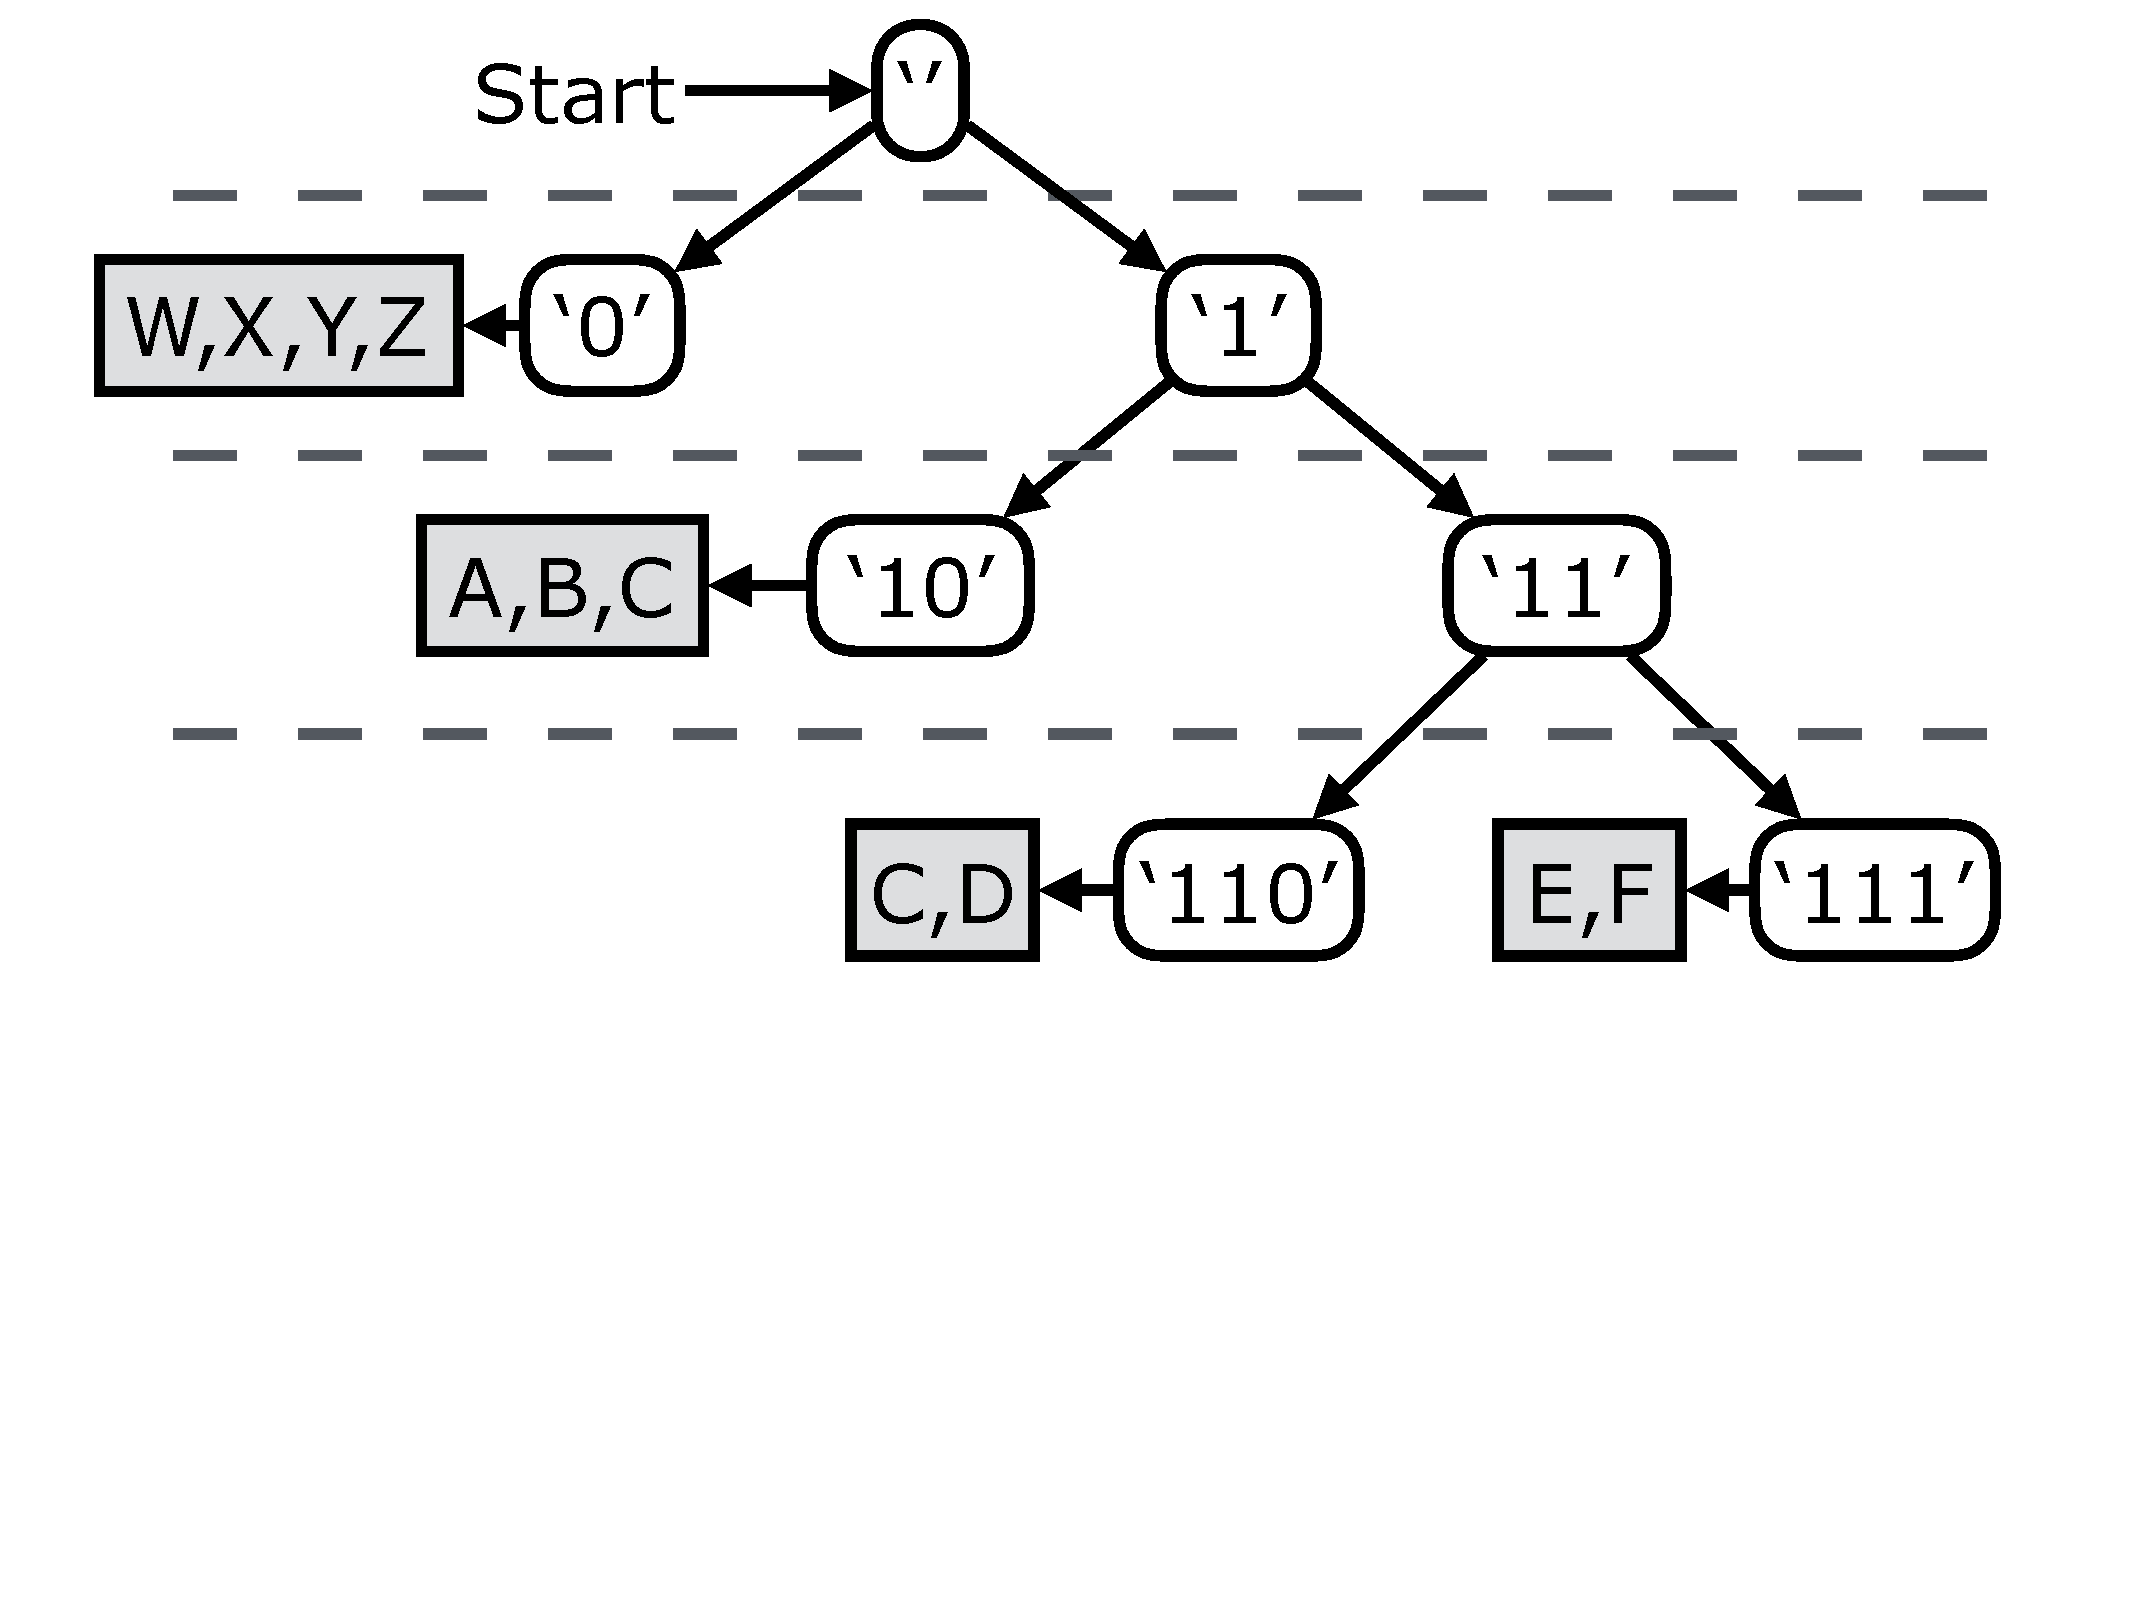
\includegraphics[trim={0 10cm 0 0}, clip, width=\linewidth]{figures/code_tree}
\end{minipage} 
\caption{An example prefix code tree, based upon the prefix code identifiers from Table~\ref{Table_variable_c} which are used to identify the attribute sets $[A,B,C]$, $[C,D]$, $[E,F]$ and $[W,X,Y,Z]$. This figure shows how reading a codeword corresponds to traversing a binary tree, starting at the root. By using such a code, larger sets are able to receive smaller identifiers, improving maximal  tag width.}
\label{fig:code_tree}
\end{figure}

\subsection{Computing Efficient Prefix Codes}
%%%
%%% Sizing the tags
%%%
Kraft's inequality~\cite{abramson} formally determines whether prefix
codes of given lengths exist.  It says that a code with $N$ codewords
of lengths $L_1, L_2, \ldots, L_N$ exists if and only if the following
inequality holds:
$$ \sum_{i = 1}^{N}{2^{-L_i}} \le 1. $$
%
For instance, the lengths of the identifiers in
Table~\ref{Table_variable}(c) 
satisfy $2^{-1} + 2^{-2} + 2^{-3} + 2^{-3} = 1$.
%
This also enables us to exactly calculate the minimal width $W_{v}$
that can be achieved for a given $N$ groups of size $\ell_1,
\ldots, \ell_N$ using variable-length identifiers as described in the
following property:

\begin{property}
For given groups of size $\ell_1, \ldots, \ell_N$ the optimal (minimal) tag width that can be derived using variable-length identifiers is given by 
\begin{equation} \label{eq2}
W_{v}  = \left \lceil \log_2 \sum_{i = 1}^{N}{2^{\ell_i}} \right \rceil. \nonumber 
\end{equation}
\label{property_variable_length_minimal_tag}
\end{property} 
\bp A width of $W_{v}$ allows assigning an identifier of length $W_{v}
- \ell_i$ to the $i$-th group. By Kraft's inequality the width $W_{v}$
must satisfy
\begin{equation} \label{eq1}
\begin{split}
1 &\ge \sum_{i = 1}^{N}{2^{-(W_{v}-\ell_i)}} = 2^{-W_{v}} \cdot \sum_{i = 1}^{N}{2^{\ell_i}}. \nonumber 
%  \Leftrightarrow 2^{W_{v}}  &\ge \sum_{i = 1}^{N}{2^{\ell_i}}  \nonumber \\
%  \Leftrightarrow W_{v}  &\ge \left \lceil \sum_{i = 1}^{N}{2^{\ell_i}}  \right \rceil \nonumber 
\end{split}
\end{equation}
Accordingly we have $2^{W_{v}}  \ge \sum_{i = 1}^{N}{2^{\ell_i}}$. Since $W_{v}$ is defined as the minimal possible width with that property, the result follows.
\ep

%In the general case, with fixed-length identifiers, given $X$ supersets of size $\ell_1, \ldots, \ell_X$ the required width is determined by the largest superset and equals 
% $W_{f} = \left \lceil \log_2(X) \right \rceil + \max_{i \in [1,X]} \ell_i$. 
 
Since the fixed-length group identifier is a special case of the
variable-length identifiers, then necessarily $W_{v} \le W_{f}$.

A selection of variable-length group identifiers satisfying Kraft's inequality can be described as a subset of leaves in a binary tree. 
A path from the root node to a node corresponds to a binary string where visits of the left child or the right child of a node stand for bits of 0 and 1, respectively. 
The path length  to a leaf corresponds to the identifier length in bits.
Figure~\ref{fig:code_tree} illustrates the corresponding tree for the four identifiers from Table~\ref{Table_variable}(c).
Shorter identifiers appear more to the left in the tree.

For given groups, after calculating $W_{v}$ as the minimal possible width enabled by variable-length identifiers, we can easily find identifiers that realize it. We first calculate for a group of size $\ell_i$ the (maximal) allowed length $W_{v} - \ell_i$. We sort the identifiers in an ascending length order. We consider a binary tree and while beginning from the root node, we relate to the next identifier the most left available leaf that its depth equals the length of the current identifier. We assign as the identifier the binary string obtained by the path from the root to the leaf.
 
\subsection{Optimizing the Selection of Groups}
In the selection of the groups, we would like to enable the existence
of as short a tag as possible. By Property~\ref{property_variable_length_minimal_tag} the number of groups and their identifiers should be selected such that their sizes $\ell_1, \ldots, \ell_N$ minimize the term $T = \sum_{i = 1}^{N}{2^{\ell_i}}$. 

We begin with the input list of attribute groups $\SS = s_1, \ldots, s_N$.
Next,  we consider each pair of groups, and calculate the benefit to the term $T$ if that pair of groups were to be replaced by their union, decreasing the number of groups by 1. For two groups $s_i, s_j$ of 
size $\ell_i, \ell_j$ and intersection size $\ell_{ij}$, the impact to $T$ of replacing them with their union $s_i \bigcup s_j$ is equal to $-2^{\ell_i} - 2^{\ell_j} + 2^{\ell_{ij}}$. However, it may be the case that no pair of groups has an impact less than 0. In such a case, we choose the pair which has minimum impact to $T$, and replace them with their union anyway. We do this because it may be the case that such a step will enable beneficial union steps later on. After each union, we record the current value of $T$ and the set of groups $\SS$ that achieved this value. This process is repeated until there is only one group remaining. 
After one group remains, we go back and identify the set of groups $\SS$ that achieved the minimum value of $T$, and return this as our answer.